\pagebreak

\section{Modelo físico}
\subsection{Implementación}

Se construyó un péndulo simple empleando 
el paquete de construcción de LEGO Mindstorms.
Este paquete posee varias características
útiles para el estudio del sistema:
\begin{itemize}
 \item Unidad de computación integrada y programable.
 \item Modularidad de sus piezas.
 \item Facilidad de ensamble.
 \item Motores de corriente directa incluyen 
 codificadores rotatorios para retroalimentación.
\end{itemize}

\subsection{Calibración del simulador}
Los parámetros de simulación fueron actualizados con las mediciones de
longitud y masa del péndulo.
La medición de masa fue realizada en dos partes debido a las limitaciones 
de capacidad de la báscula analítica\footnote{Mettler Toledo MS104TS/00}.
La masa total del péndulo resultó ser de 0.1232109 kilogramos.
Para determinar la longitud efectiva del péndulo, se identificó de manera 
experimental el centro de masas del péndulo.
Empleando el método de balance de momentos, se identificó que el 
centro de masa estaba ubicado aproximadamente a 0.193 metros 
del punto de unión con la junta rotacional.\\

\subsection{Caída libre del péndulo}

Empleando los sensores incluidos en el paquete de LEGO
Mindstorms, fue posible realizar mediciones de la 
posición angular del péndulo para comparar con el
modelo matemático y el análisis de video.
La figura \ref{fig: mindstorms theta} muestra la
gráfica de mediciones de $\theta$ respecto al tiempo.
Se observa que las mediciones realizadas por el sensor
fueron afectadas por el nivel de ruido introducido 
por el mismo sensor.

\begin{figure}[htb!]
 \centering
\import{./img/}{lego.tex}
 \caption{Mediciones de $\theta$ para el péndulo físico con el codificador rotatorio.}
 \label{fig: mindstorms theta}
\end{figure}

\subsubsection{Función de decaimiento}

Se realizó una regresión cuadrática de las mediciones obtenidas con el propósito de 
identificar la ecuación de decaimiento del sistema.
Empleando las herramientas de ajuste de curva de MATLAB se obtuvo una función polinomial
de segundo orden para el tiempo de estabilización del sistema.
La figura \ref{fig: regresion} presenta el ajuste de curvas efectuado.

\begin{equation}
 y = 1.2 x^2 - 21 x + 86
\end{equation}

\begin{figure}[htb!]
 \centering
%  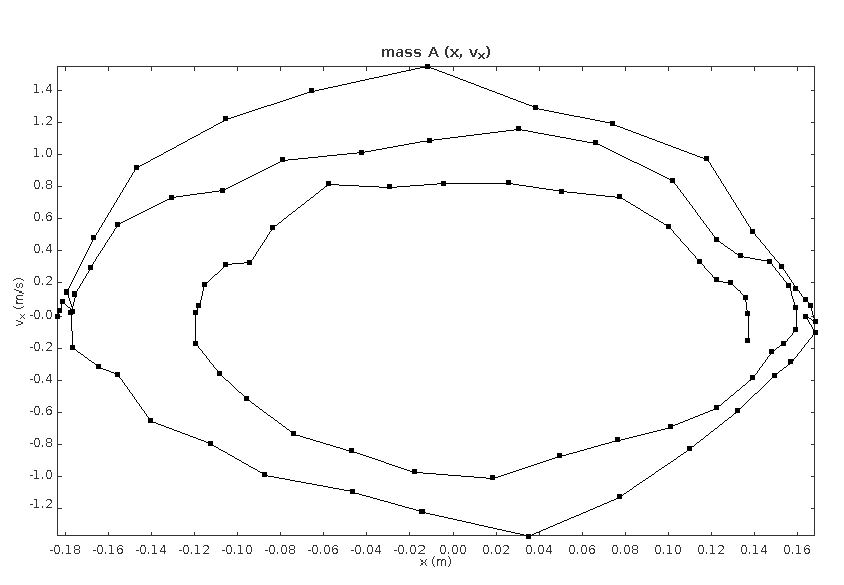
\includegraphics[scale=0.4]{./img/tracker_poc_phasediagram_x_vx.png}
\import{./img/}{regresion.pdf_tex}
 % tracker_poc_phasediagram_x_vx.png: 844x585 px, 72dpi, 29.78x20.64 cm, bb=0 0 844 585
 \caption{Función de decaimiento del sistema.}
 \label{fig: regresion}
\end{figure}

\pagebreak

\subsection{Análisis de video}

Se realizó un análisis de video del péndulo con 
el software de \emph{Tracker}\footnote{\url{https://www.physlets.org/tracker/}}.
El video fue grabado a 30 cuadros por segundo (fps) en resolución HD.
Empleando las herramientas de procesamiento de imagen, rastreo de imagen y 
 medición de propiedades físicas fue posible 
obtener información detallada del movimiento lineal y rotacional del sistema.
Esta información fue almacenada en archivo CSV para procesarla 
en Octave y poder realizar una comparación del modelo matemático planteado y 
el comportamiento del sistema real.

Empleando Tracker, fue posible generar diagramas de fase de la 
posición, velocidad y aceleración del sistema.
Estas mediciones pudieron ser realizados tanto para el movimiento lineal del
péndulo como para su movimiento angular.
La figura \ref{fig: tracker theta} presenta el diagrama de la posición angular 
del péndulo respecto al tiempo total de operación.
Se observa que el péndulo experimenta una pérdida de energía considerable 
en cada período de oscilación.
Se presenta también el diagrama de fase 
(figura \ref{fig: tracker phase diagram theta dtheta})
para el desplazamiento y velocidad angular del péndulo.
La curva generada concuerda con las gráficas generadas en 
la sección \ref{simulation friction}.

Estos resultados ya dan una indicación sobre la certeza del simulador.
El movimento del péndulo real y la simulación indican ser similares.
No obstante, esta primer comparación no permite conocer con certeza 
detalles más relevantes sobre el péndulo como la frecuencia de oscilación.

\begin{figure}[htb!]
 \centering
%  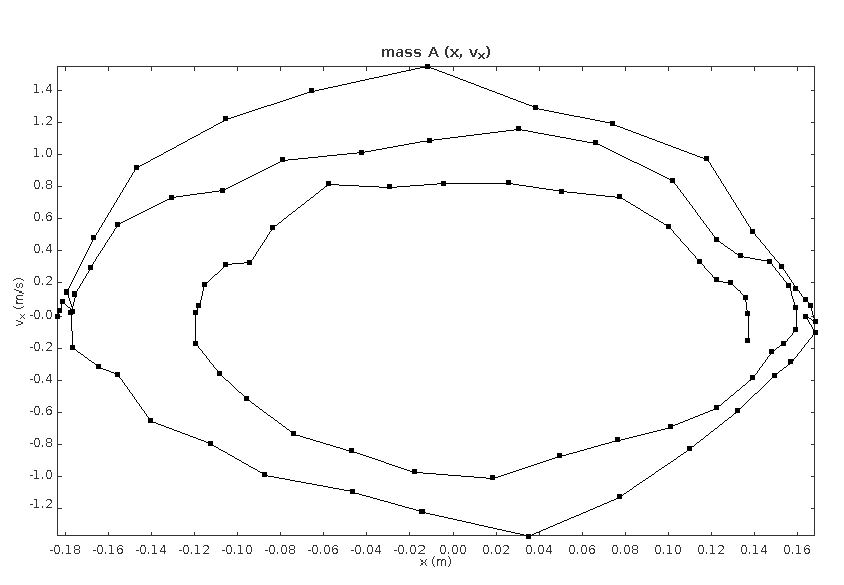
\includegraphics[scale=0.4]{./img/tracker_poc_phasediagram_x_vx.png}
\import{./img/}{pendulum_theta_tracker.pdf_tex}
 % tracker_poc_phasediagram_x_vx.png: 844x585 px, 72dpi, 29.78x20.64 cm, bb=0 0 844 585
 \caption{Posición angular del sistema.}
 \label{fig: tracker theta}
\end{figure}



\begin{figure}[htb!]
\centering
%  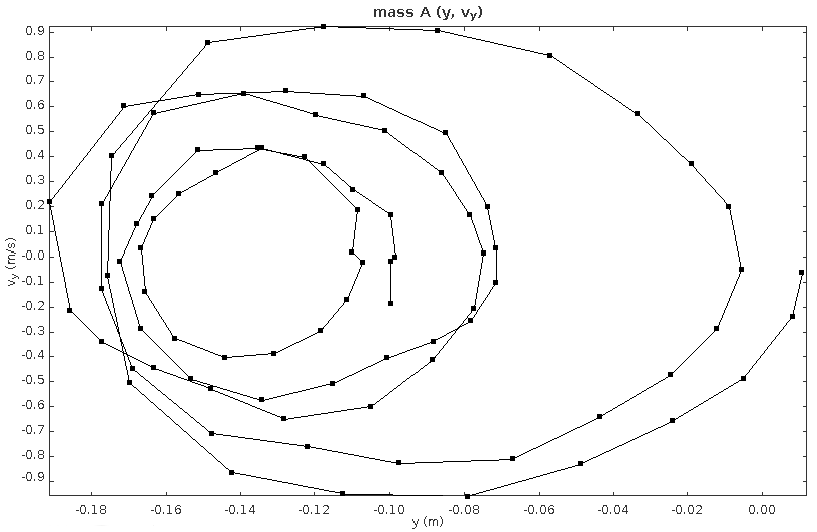
\includegraphics[scale=0.4]{./img/tracker_poc_phasediagram_y_vy.png}
\import{./img/}{pendulum_phase_tracker.pdf_tex}
% tracker_poc_phasediagram_x_vx.png: 844x585 px, 72dpi, 29.78x20.64 cm, bb=0 0 844 585
\caption{Diagrama de fase del modelo físico para $\theta$ y $\dot \theta$.}
\label{fig: tracker phase diagram theta dtheta}
\end{figure}

\pagebreak

\subsection{Comparación con el modelo matemático}
Utilizando las mediciones obtenidas con el análisis de video fue posible hacer 
comparaciones más detalladas sobre ambos sistemas.
Las figura \ref{fig: tracker friction theta} y \ref{fig: tracker friction dtheta}
muestran la comparación de la posición angular $\theta$ 
y velocidad angular $\theta$ para las condiciones de simulación descritas
con anterioridad.
Es evidente que el modelo matemático describe un comportamiento similar al 
péndulo real.
No obstante, los valores de frecuencia y amplitud que se observan para ambas curvas
difieren considerablemente.
La diferencia en frecuencia de oscilación indica que la longitud efectiva 
del péndulo no concuerda con el modelo real.
La diferencia en decaimiento de la amplitud del sistema se atribuye a un valor 
inapropiado del coeficiente de fricción.

\begin{figure}[htb!]
 \centering
%  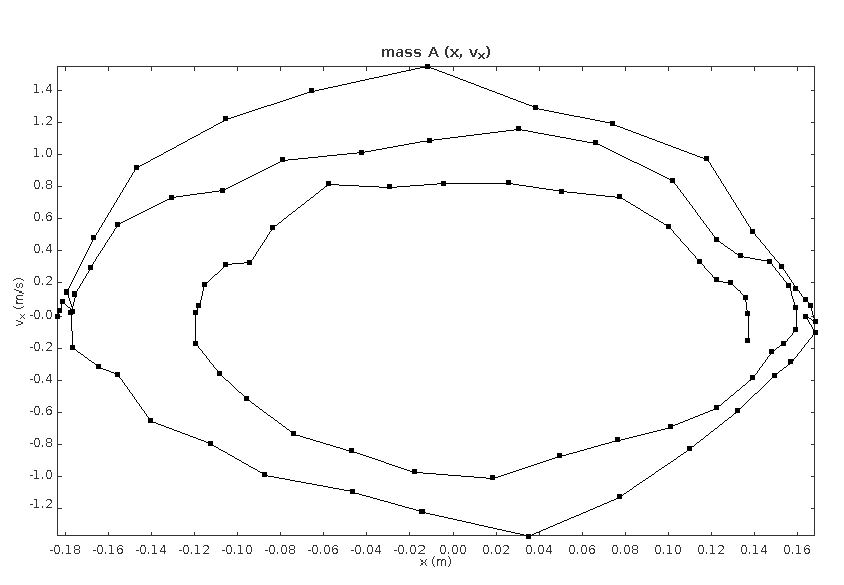
\includegraphics[scale=0.4]{./img/tracker_poc_phasediagram_x_vx.png}
\import{./img/}{trackerTheta.tex}
 % tracker_poc_phasediagram_x_vx.png: 844x585 px, 72dpi, 29.78x20.64 cm, bb=0 0 844 585
 \caption{Comparación de la posición angular del sistema simulado y real.}
 \label{fig: time tracker theta}
\end{figure}

\begin{figure}[htb!]
\centering
%  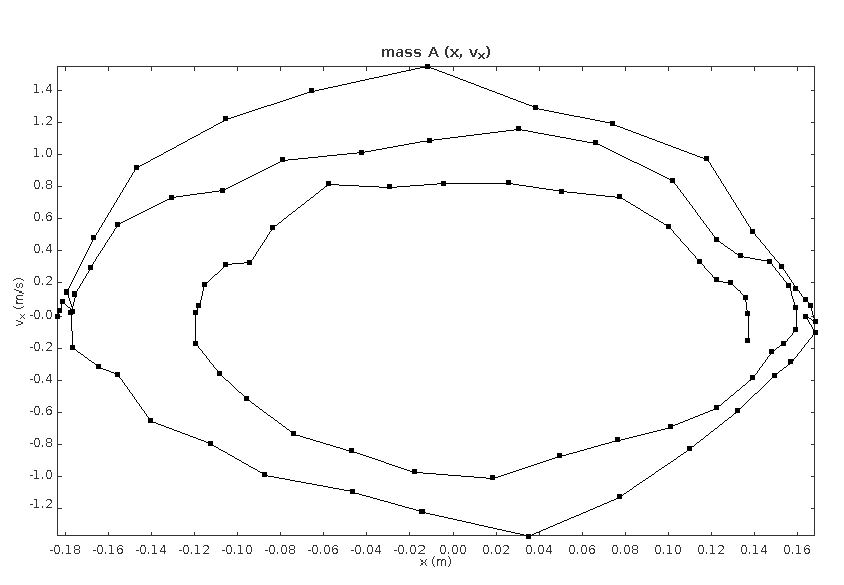
\includegraphics[scale=0.4]{./img/tracker_poc_phasediagram_x_vx.png}
\import{./img/}{trackerdTheta.tex}
% tracker_poc_phasediagram_x_vx.png: 844x585 px, 72dpi, 29.78x20.64 cm, bb=0 0 844 585
\caption{Comparación de la velocidad angular del sistema simulado y real.}
\label{fig: time tracker dtheta}
\end{figure}

\subsubsection{Coeficiente de fricción viscosa}
Para determinar un nuevo valor para el coeficiente de fricción se realizaron 
simulaciones con un total de 20 nuevos valores, incrementando en intervalos de
0.05 respecto al valor original.
Las figuras \ref{fig: time tracker theta friction} y 
\ref{fig: time tracker dtheta friction} muestran el nuevo
comportamiento del sistema para el valor seleccionado del coeficiente
de fricción viscosa $k = 0.135$.


\begin{figure}[htb!]
 \centering
%  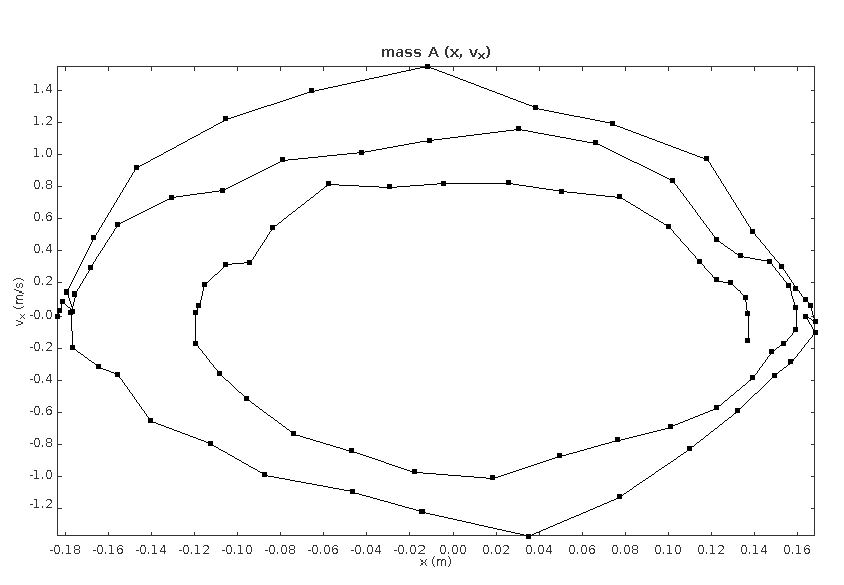
\includegraphics[scale=0.4]{./img/tracker_poc_phasediagram_x_vx.png}
\import{./img/}{trackerThetaF.tex}
 % tracker_poc_phasediagram_x_vx.png: 844x585 px, 72dpi, 29.78x20.64 cm, bb=0 0 844 585
 \caption{Posición angular para el nuevo valor del coeficiente de fricción $k = 0.135$.}
 \label{fig: time tracker theta friction}
\end{figure}

\begin{figure}[htb!]
 \centering
%  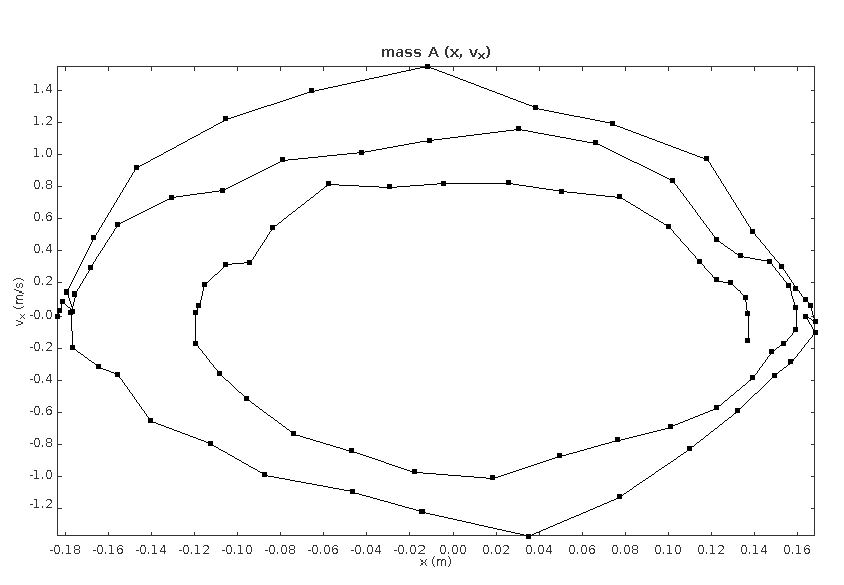
\includegraphics[scale=0.4]{./img/tracker_poc_phasediagram_x_vx.png}
\import{./img/}{trackerdThetaF.tex}
 % tracker_poc_phasediagram_x_vx.png: 844x585 px, 72dpi, 29.78x20.64 cm, bb=0 0 844 585
 \caption{Velocidad angular para el nuevo valor del coeficiente de fricción $k = 0.135$.}
 \label{fig: time tracker dtheta friction}
\end{figure}

\subsubsection{Longitud efectiva del péndulo}
Se obtuvo una nueva longitud efectiva del péndulo de manera similar al 
coeficiente de fricción. 
La nueva longitud efectiva del péndulo fue seleccionada a manera de que el 
modelo simulado oscilara en la misma frecuencia que el sistema real, o lo 
más cercano posible a esta.
Las figuras \ref{fig: time tracker theta new length} y 
\ref{fig: time tracker dtheta new length} muestran el comportamiento del simulador
con los nuevos valores del coeficiente de fricción y longitud efectiva del péndulo.

\begin{figure}[htb!]
 \centering
%  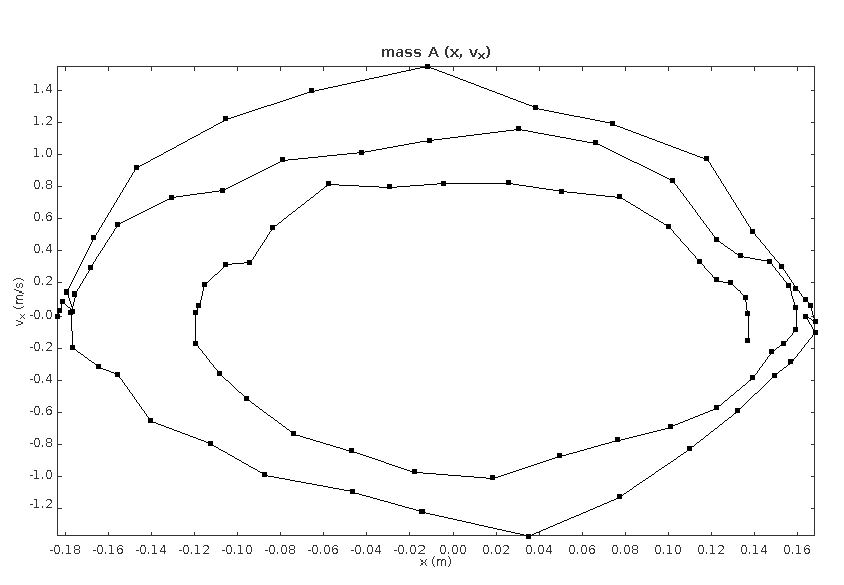
\includegraphics[scale=0.4]{./img/tracker_poc_phasediagram_x_vx.png}
\import{./img/}{trackerThetaL.tex}
 % tracker_poc_phasediagram_x_vx.png: 844x585 px, 72dpi, 29.78x20.64 cm, bb=0 0 844 585
 \caption{Posición angular para el nuevo valor de longitud $l = 0.22 [m]$.}
 \label{fig: time tracker theta new length}
\end{figure}

\begin{figure}[htb!]
 \centering
%  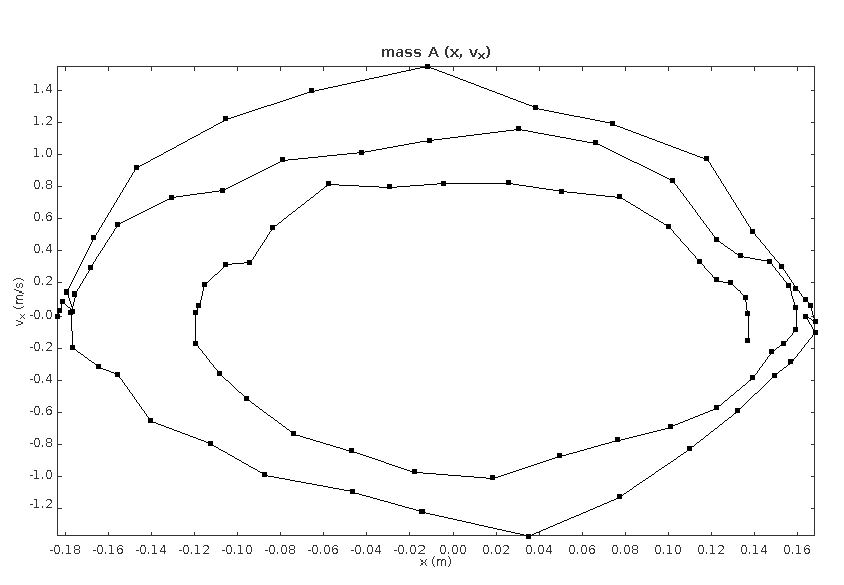
\includegraphics[scale=0.4]{./img/tracker_poc_phasediagram_x_vx.png}
\import{./img/}{trackerdThetaL.tex}
 % tracker_poc_phasediagram_x_vx.png: 844x585 px, 72dpi, 29.78x20.64 cm, bb=0 0 844 585
 \caption{Velocidad angular para el nuevo valor de longitud $l = 0.22 [m]$.}
 \label{fig: time tracker dtheta new length}
\end{figure}



\clearpage
